\begin{frame} \frametitle{\textit{Past work}: Efficient estimation of the probability density function of transmission loss in uncertain ocean environments}
  {\small
    \vspace*{0.25cm}
    Transmission Loss, $TL=20log_{10}\left(\frac{p_{source}}{p_{receiver}}\right)$, is useful for naval applications.
    \vspace*{0.25cm}
    \begin{figure}
      \centering
      \begin{tikzpicture}
        \node[anchor=south west,inner sep=0] (image) at (0,0) {
          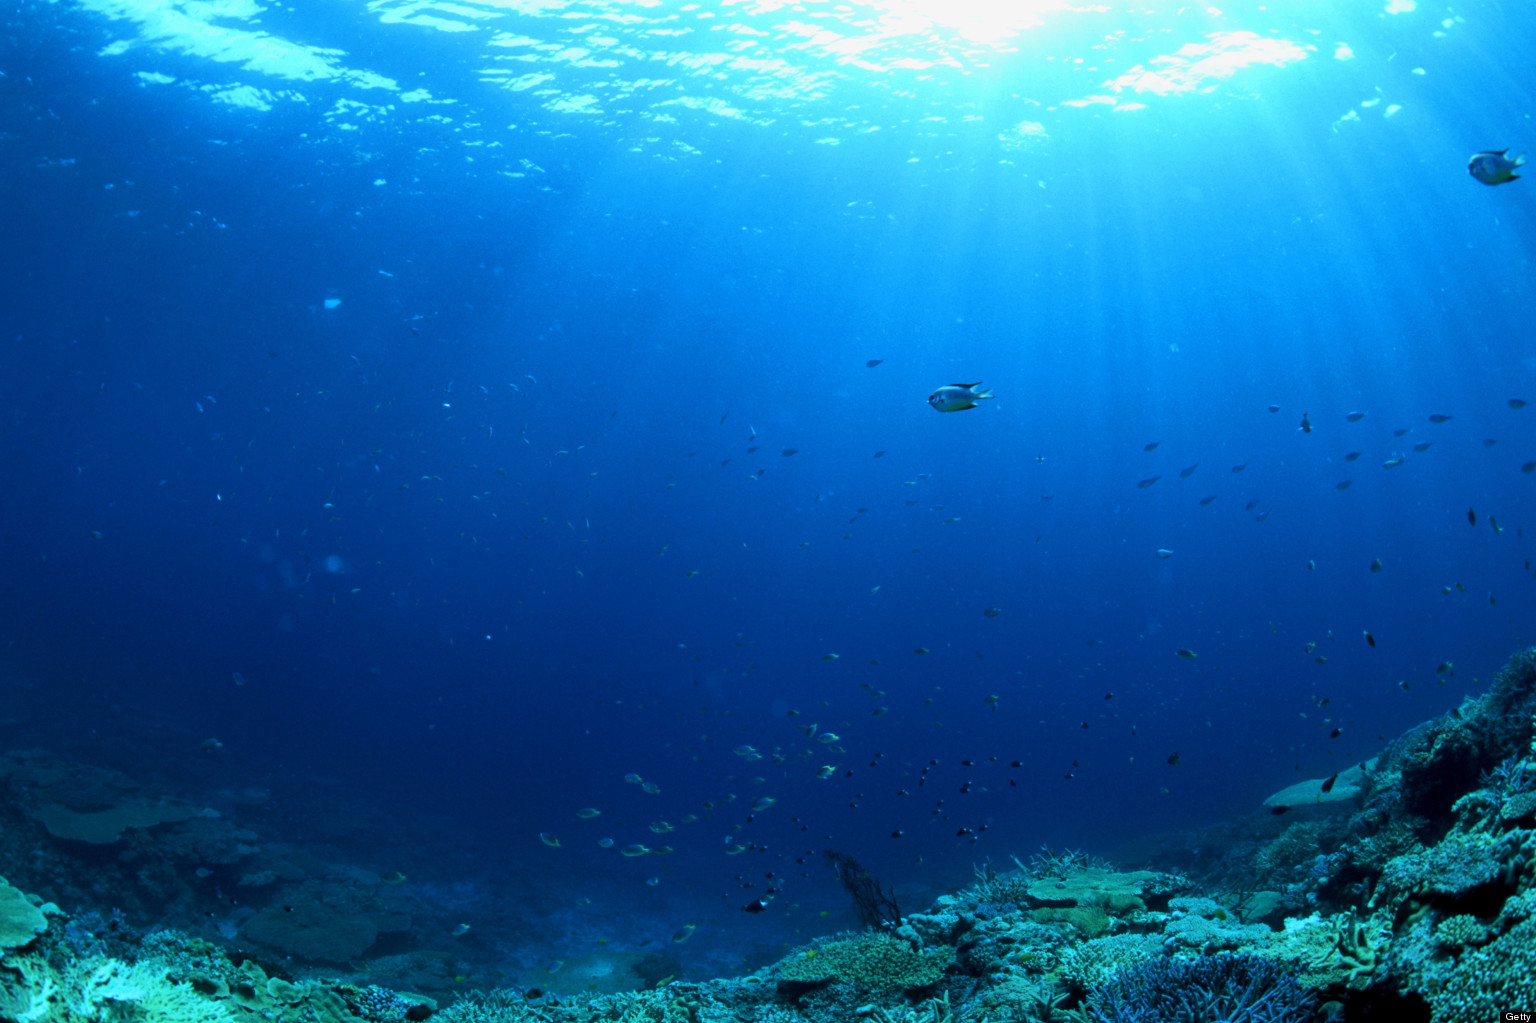
\includegraphics[width=0.6\textwidth]{./figs/ocean_0}
        };%
        \begin{scope}[x={(image.south east)},y={(image.north west)}]%
          \node[font=\tiny,right] at (0.9,0.03) {\textcolor{white}{Getty Images}};%
        \end{scope}%  
      \end{tikzpicture}%
    \end{figure}
    TL uncertainty is important for those making decisions based on TL,
    but traditional methods are slow and expensive.}
  %
  \note{
    \begin{enumerate}
    \item TL is essentially a measure of how much quieter sound has gotten since leaving its source. 
    \item In the ocean TL is useful in a variety of practical naval applications and can be approximately calculated if the environment is perfectly known.
    \item The ocean has a lot going on.
    \item People who make decisions based on TL want to know how much they can trust their TL calcs or what's the uncertainty.
    \item There are established ways of doing this. MC is the gold standard. But MC and the other ways are computationally expensive.
    \item I developed a computationally efficient way of calculating TL uncertainty.
    \end{enumerate}
  }
\end{frame}
%% 
%% 
\begin{frame} \frametitle{\textit{Past work}: We developed a computationally efficient way of computing TL in uncertain environments}
  \begin{figure}\hfill
    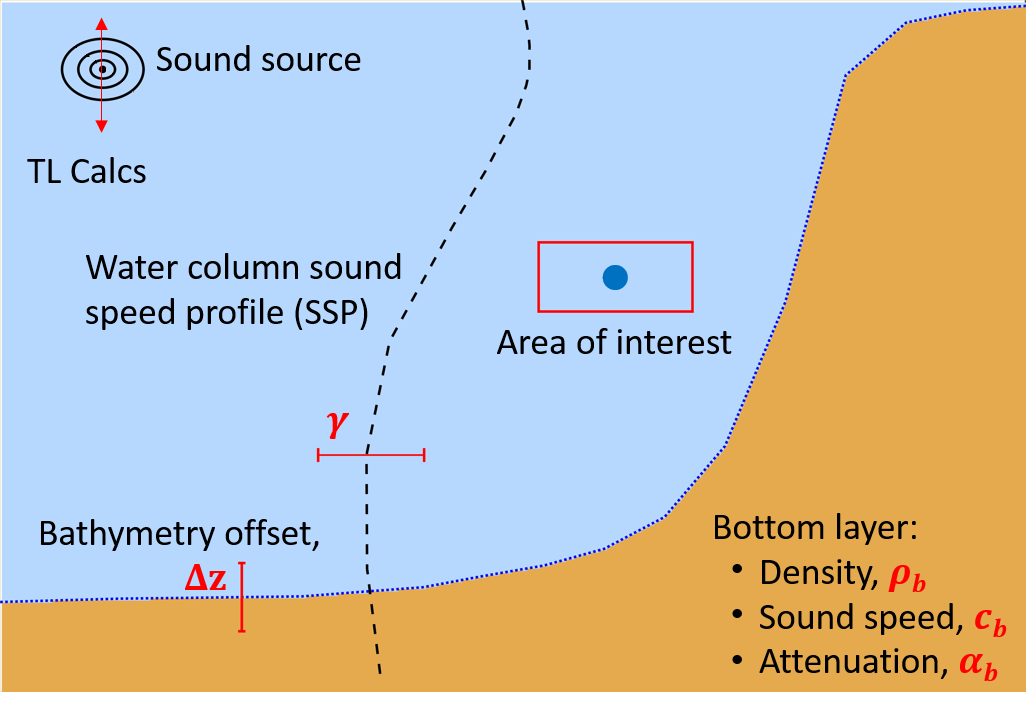
\includegraphics[height=0.3\textheight]{./figs/as_ocean_schematic}\hfill
    \visible<2->{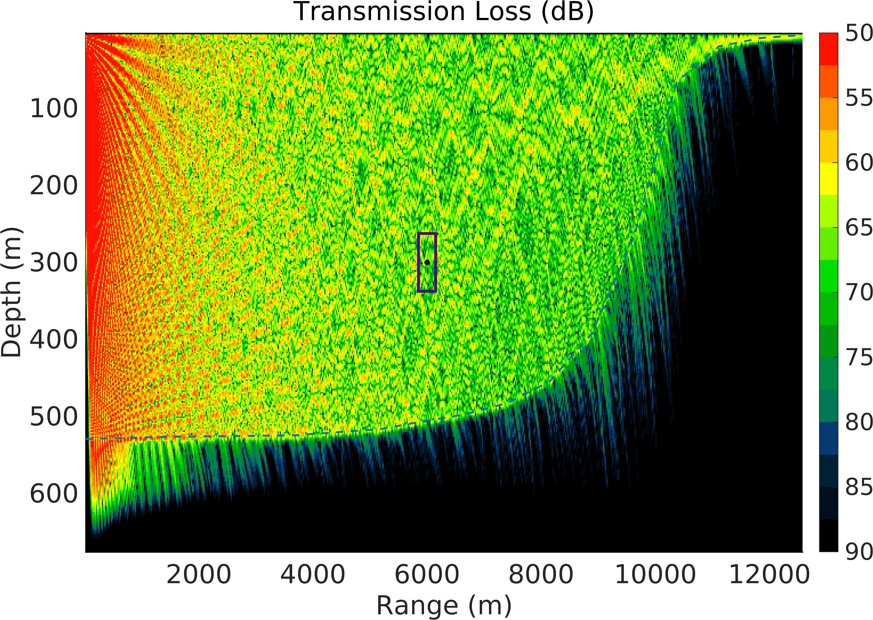
\includegraphics[height=0.32\textheight]{./figs/as_field}}\hfill
    \visible<3->{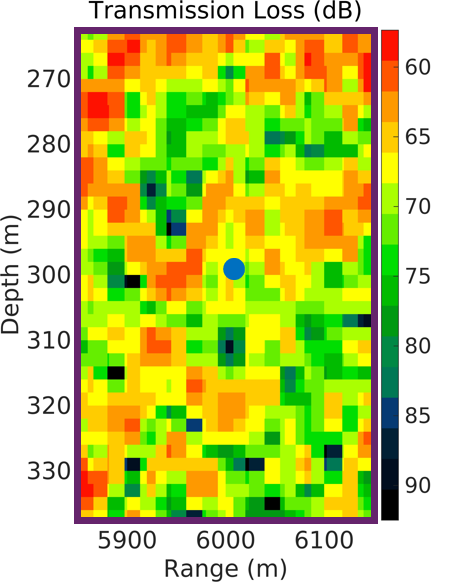
\includegraphics[height=0.32\textheight]{./figs/as_subfield}}\hfill
  \end{figure}
  \vspace{-0.7cm}
  \begin{figure}
    \visible<4->{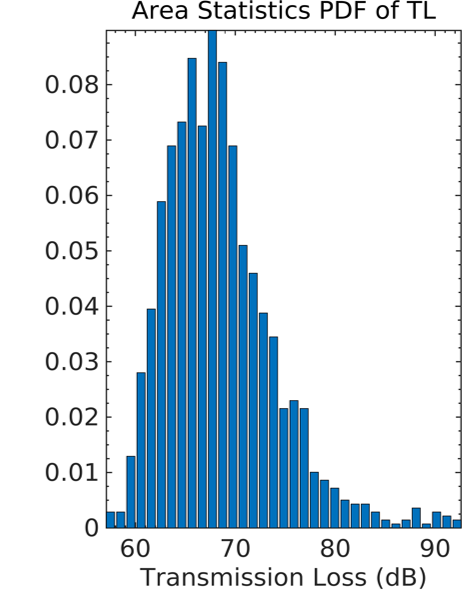
\includegraphics[height=0.3\textheight]{./figs/as_hist}}\hfill
    \visible<5->{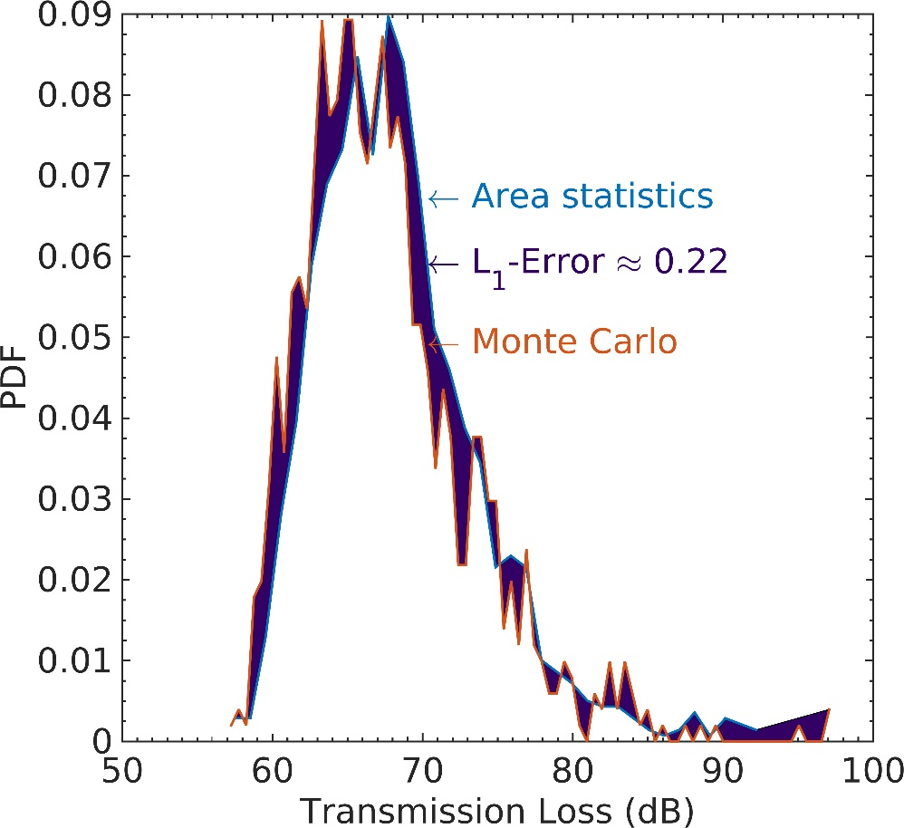
\includegraphics[height=0.3\textheight]{./figs/as_mc_tlpdf}}\hfill
    \visible<6->{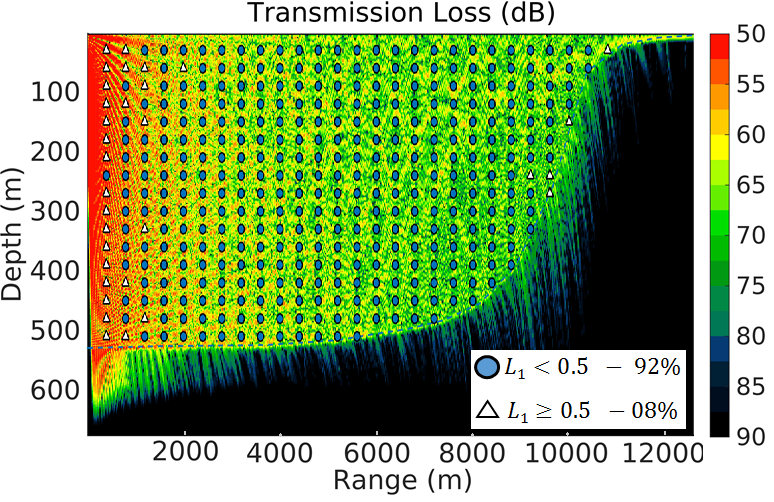
\includegraphics[height=0.32\textheight]{./figs/tl_success_field_labeled}}\hfill
  \end{figure}
  \vspace{-0.5cm}
  {\footnotesize
    \visible<7->{
      \begin{itemize}
      \item Engineering level accurate $\left(L_1\text{-error}<0.5\right)$ in 93\% of test cases in bottom reflecting environments. \vspace*{-4pt}
      \item $\approx \orderof{10^{-6}}$ the cost of 1000-sample Monte Carlo Methods.
      \end{itemize}
    }
  }
  \note{To Do: Find higher quality version of last figure}
  \note{Mauro's questions:\\(1) What is shallow?\\(2) How does the functional depth of this technique compare to important depths for relevant applications?}
\end{frame}
%
%%% Local Variables:
%%% mode: latex
%%% TeX-master: ../main
%%% End:
